\section{Thống kê suy diễn}
\subsection{Anova một nhân tố: So sánh tổng chi phí đặt hàng theo mùa}
Ta sẽ tách dữ liệu theo mùa (\textbf{Code[180$\to$183]}). Các giả định cần kiểm tra:
\begin{itemize}
    \item[+] Tổng chi phí đặt hàng ở các mùa tuân theo phân phối chuẩn.
    \item[+] Phương sai tổng chi phí đặt hàng ở các mùa bằng nhau.
\end{itemize}
\subsubsection*{Kiểm định giả định về phân phối chuẩn:}
%%%%%%%%%%%%%%%%%%%%%%%%%%%%%%%%%%%%%%%%%%%%%%%%%%%%%%%%%%%%%%%%%%%%%%%%%%%%%%%%%%

\textbf{\textit{Đối với mùa xuân}}, ta thực hiện vẽ đồ thị(\textbf{Code[185$\to$186]}): 
\begin{figure}[H]
    \centering
    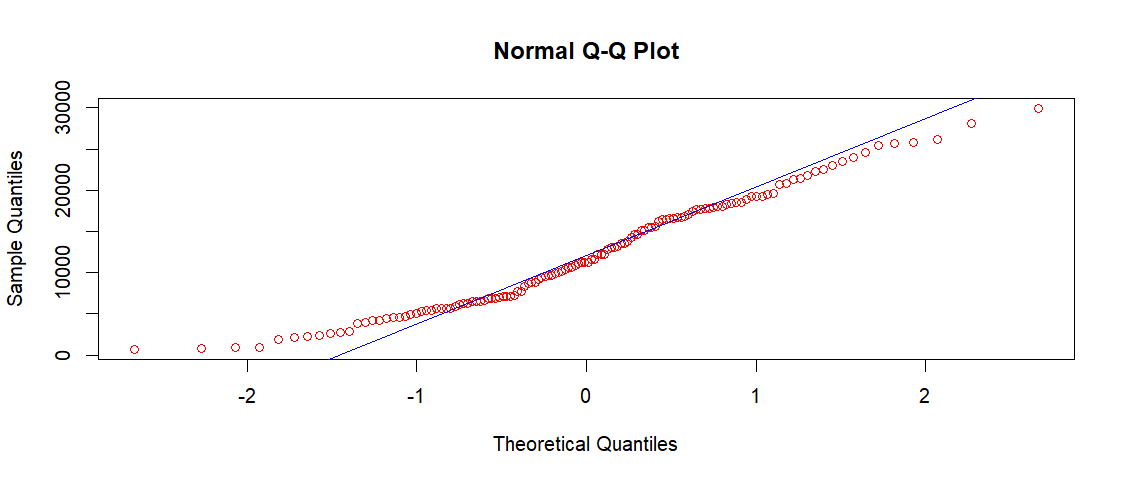
\includegraphics[width = 0.8\textwidth]{IMAGES/25.png}
    \caption{Kết quả khi vẽ Normal QQ-plot cho order\_total theo mùa xuân}
    \label{fig29}
\end{figure}

\textbf{Nhận xét:} Hình~\ref{fig29} cung cấp đồ thị QQ để so sánh phân phối của dữ liệu với phân phối chuẩn. Dựa vào đồ thị QQ-plot ta thấy các quan trắc nằm lệch ra khỏi đường thẳng kỳ vọng phân phối chuẩn nên có thể kết luận tổng chi phí đặt hàng ở mùa xuân không tuân theo phân phối chuẩn.

Ngoài ra, ta có thể dùng hàm Shapiro.test để kiểm tra:
\begin{itemize}
    \item[] Giả thuyết H$_0$: Chi phí đặt hàng ở mùa xuân tuân theo phân phối chuẩn.
    \item[] Đối thuyết H$_1$: Chi phí đặt hàng ở mùa xuân không tuân theo phân phối chuẩn.
\end{itemize}
\textbf{Code[187]}

\begin{figure}[H]
    \centering
    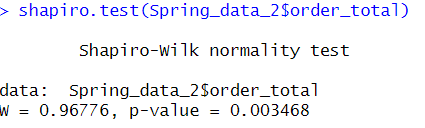
\includegraphics[width = 0.5\textwidth]{IMAGES/26.png}
    \caption{Kết quả khi dùng kiểm định Shapiro.test cho order\_total theo mùa xuân}
    \label{fig30}
\end{figure}

\textbf{Nhận xét:} Hình~\ref{fig30} Kết quả của phương pháp Shapiro test được trình bày trong hình~\ref{fig30}, dựa vào p-value  = $0.0035$ $<$ mức ý nghĩa $5\%$ ở kiểm định Shapiro.test nên ta bác bỏ H$_0$ và chấp nhận H$_1$. Vậy tổng chi phí đặt hàng ở mùa xuân không tuân theo phân phối chuẩn.

%%%%%%%%%%%%%%%%%%%%%%%%%%%%%%%%%%%%%%%%%%%%%%%%%%%%%%%%%%%%%%%%%%%%%%%%%%%%%%%%%%
\textbf{\textit{Đối với mùa hạ}}, ta thực hiện vẽ đồ thị(\textbf{Code[189$\to$190]}): 
\begin{figure}[H]
    \centering
    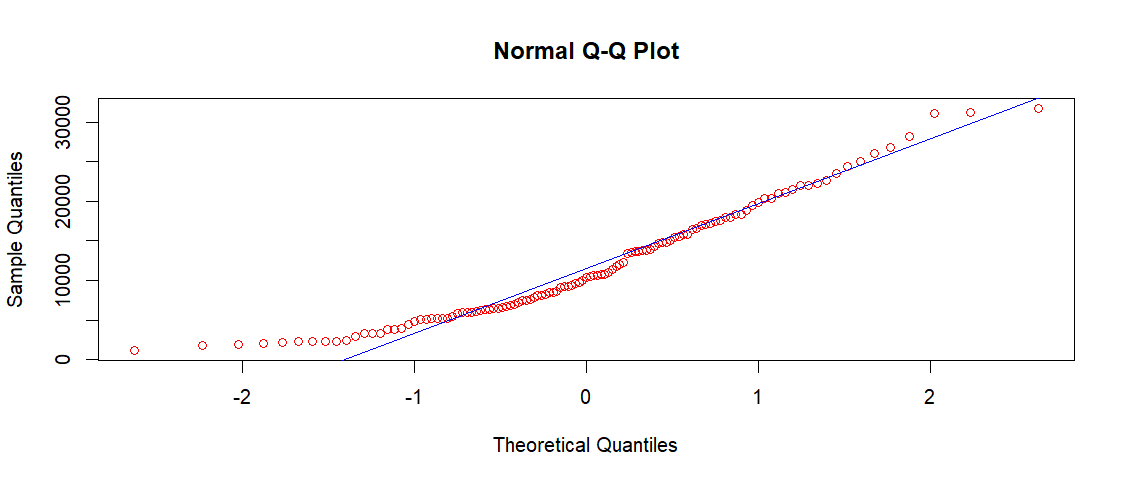
\includegraphics[width = 0.8\textwidth]{IMAGES/27.png}
    \caption{Kết quả khi vẽ Normal QQ-plot cho order\_total theo mùa hạ}
    \label{fig31}
\end{figure}

\textbf{Nhận xét:} Hình~\ref{fig31} cung cấp cho ta đồ thị QQ để so sánh phân phối của dữ liệu với phân phối chuẩn. Dựa vào đồ thị QQ-plot ta thấy các quan trắc nằm lệch ra khỏi đường thẳng kỳ vọng phân phối chuẩn nên có thể kết luận tổng chi phí đặt hàng ở mùa hạ không tuân theo phân phối chuẩn.

Ngoài ra, ta có thể dùng hàm Shapiro.test để kiểm tra:
\begin{itemize}
    \item[] Giả thuyết H$_0$: Chi phí đặt hàng ở mùa hạ tuân theo phân phối chuẩn.
    \item[] Đối thuyết H$_1$: Chi phí đặt hàng ở mùa hạ không tuân theo phân phối chuẩn.
\end{itemize}
\textbf{Code[191]}

\begin{figure}[H]
    \centering
    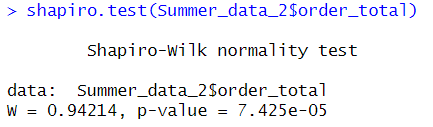
\includegraphics[width = 0.6\textwidth]{IMAGES/28.png}
    \caption{Kết quả khi dùng kiểm định Shapiro.test cho order\_total theo mùa hạ}
    \label{fig32}
\end{figure}
\textbf{Nhận xét:} Hình~\ref{fig32} Kết quả của phương pháp Shapiro test được trình bày trong hình~\ref{fig32}, dựa vào p-value  = $7.425e-05$ $<$ mức ý nghĩa $5\%$ ở kiểm định Shapiro.test nên ta bác bỏ H$_0$ và chấp nhận H$_1$. Vậy tổng chi phí đặt hàng ở mùa hạ không tuân theo phân phối chuẩn.
%%%%%%%%%%%%%%%%%%%%%%%%%%%%%%%%%%%%%%%%%%%%%%%%%%%%%%%%%%%%%%%%%%%%%%%%%%%%%%%%%%

\textbf{\textit{Đối với mùa thu}}, ta thực hiện vẽ đồ thị (\textbf{Code[193$\to$194]}): 
\begin{figure}[H]
    \centering
    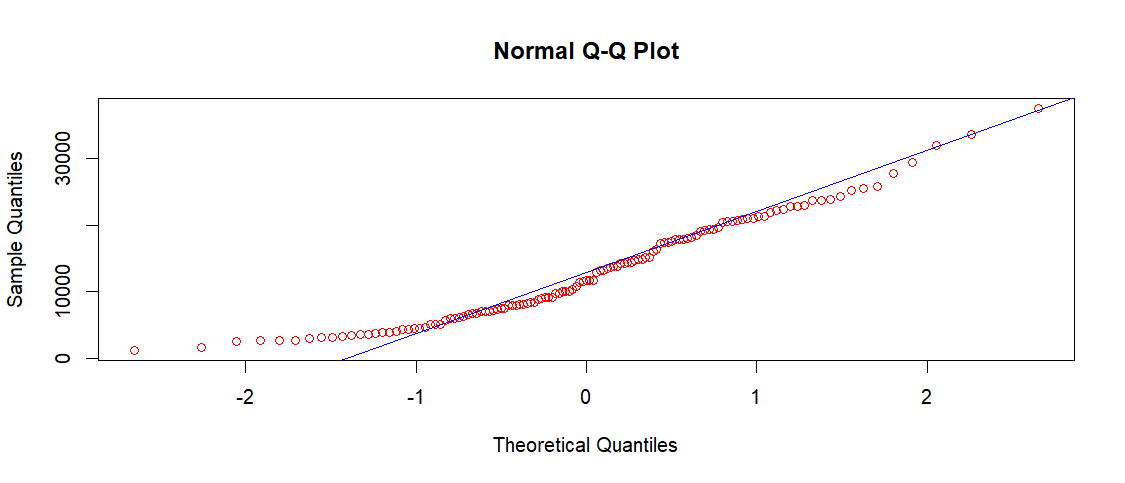
\includegraphics[width = 0.8\textwidth]{IMAGES/29.png}
    \caption{Kết quả khi vẽ Normal QQ-plot cho order\_total theo mùa thu}
    \label{fig33}
\end{figure}

\textbf{Nhận xét:} Hình~\ref{fig33} cung cấp cho ta đồ thị QQ để so sánh phân phối của dữ liệu với phân phối chuẩn. Dựa vào đồ thị QQ-plot ta thấy các quan trắc nằm lệch ra khỏi đường thẳng kỳ vọng phân phối chuẩn nên có thể kết luận tổng chi phí đặt hàng ở mùa thu không tuân theo phân phối chuẩn.

Ngoài ra, ta có thể dùng hàm Shapiro.test để kiểm tra:
\begin{itemize}
    \item[] Giả thuyết H$_0$: Chi phí đặt hàng ở mùa thu tuân theo phân phối chuẩn.
    \item[] Đối thuyết H$_1$: Chi phí đặt hàng ở mùa thu không tuân theo phân phối chuẩn.
\end{itemize}
\textbf{Code[195]}

\begin{figure}[H]
    \centering
    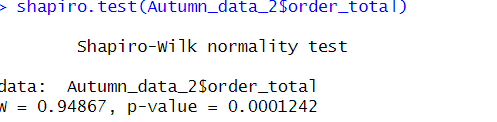
\includegraphics[width = 0.6\textwidth]{IMAGES/30.png}
    \caption{Kết quả khi dùng kiểm định Shapiro.test cho order\_total theo mùa thu}
    \label{fig34}
\end{figure}
\textbf{Nhận xét:} Kết quả của phương pháp Shapiro test được trình bày trong hình~\ref{fig34}, dựa vào p-value  = $0.0001242$ $<$ mức ý nghĩa $5\%$ ở kiểm định Shapiro.test nên ta bác bỏ H$_0$ và chấp nhận H$_1$. Vậy tổng chi phí đặt hàng ở mùa thu không tuân theo phân phối chuẩn.
%%%%%%%%%%%%%%%%%%%%%%%%%%%%%%%%%%%%%%%%%%%%%%%%%%%%%%%%%%%%%%%%%%%%%%%%%%%%%%%%%%

\textbf{\textit{Đối với mùa đông}}, ta thực hiện vẽ đồ thị (\textbf{Code[197$\to$198]}): 
\begin{figure}[H]
    \centering
    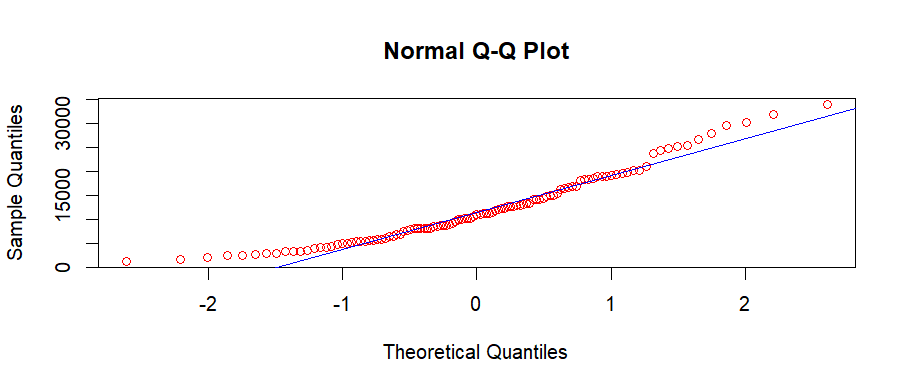
\includegraphics[width = 0.8\textwidth]{IMAGES/31.png}
    \caption{Kết quả khi vẽ Normal QQ-plot cho order\_total theo mùa đông}
    \label{fig35}
\end{figure}
\textbf{Nhận xét:} Hình~\ref{fig35} cung cấp cho ta đồ thị QQ để so sánh phân phối của dữ liệu với phân phối chuẩn. Dựa vào đồ thị QQ-plot ta thấy các quan trắc nằm lệch ra khỏi đường thẳng kỳ vọng phân phối chuẩn nên có thể kết luận tổng chi phí đặt hàng ở mùa hạ không tuân theo phân phối chuẩn.

Ngoài ra, ta có thể dùng hàm Shapiro.test để kiểm tra:
\begin{itemize}
    \item[] Giả thuyết H$_0$: Chi phí đặt hàng ở mùa hạ tuân theo phân phối chuẩn.
    \item[] Đối thuyết H$_1$: Chi phí đặt hàng ở mùa hạ không tuân theo phân phối chuẩn.
\end{itemize}
\textbf{Code[199]}

\begin{figure}[H]
    \centering
    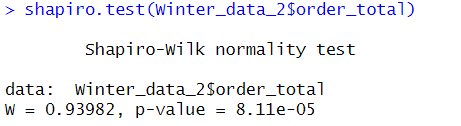
\includegraphics[width = 0.6\textwidth]{IMAGES/32.png}
    \caption{Kết quả khi dùng kiểm định Shapiro.test cho order\_total theo mùa đông}
    \label{fig36}
\end{figure}
\textbf{Nhận xét:} Kết quả của phương pháp Shapiro test được trình bày trong hình~\ref{fig36}, dựa vào p-value  = $8.11e-05$ $<$ mức ý nghĩa $5\%$ ở kiểm định Shapiro.test nên ta bác bỏ H$_0$ và chấp nhận H$_1$. Vậy tổng chi phí đặt hàng ở mùa hạ không tuân theo phân phối chuẩn.

\textbf{Kết luận:} vậy có sự khác nhau về tổng chi phí đặt hàng ở cả bốn mùa.
\subsubsection*{Kiểm định giả định về tính đồng nhất của phương sai:}
\begin{itemize}
    \item[] Giả thuyết H$_0$: Phương sai tổng chi phí đặt hàng ở các mùa bằng nhau.
    \item[] Đối thuyết H$_1$: Có ít nhất hai mùa có phương sai tổng chi phí đặt hàng khác nhau.
\end{itemize}
\textbf{Code[201$\to$202]}
\begin{figure}[H]
    \centering
    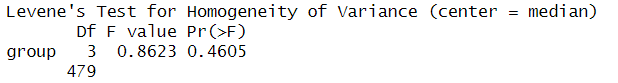
\includegraphics[width = 0.6\textwidth]{IMAGES/48.png}
    \caption{code R và kết quả khi kiểm tra giả định phương sai}
    \label{fig37}
\end{figure}

\textbf{Nhận xét:} Kết quả của phương pháp Levene test được trình bày trong hình~\ref{fig37}, dựa vào p-value = $0.4605$ $>$ mức ý nghĩa $5\%$ ở kiểm định leveneTest nên ta có thể kết luận phương sai tổng chi phí đặt hàng ở các mùa là bằng nhau.
\subsubsection*{Thực hiện Anova một nhân tố so sánh tổng chi phí đặt hàng trung bình ở các mùa:}
\begin{itemize}
    \item[] Giả thuyết H$_0$: Tổng chi phí đặt hàng trung bình ở các mùa bằng nhau.
    \item[] Đối thuyết H$_1$: Có ít nhất hai mùa có tổng chi phí đặt hàng khác nhau.
\end{itemize}
\textbf{Code[204$\to$205]}
\begin{figure}[H]
    \centering
    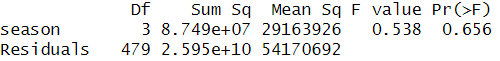
\includegraphics[width = 0.6\textwidth]{IMAGES/49.png}
    \caption{Kết quả khi thực hiện Anova một nhân tố}
    \label{fig38}
\end{figure}

\textbf{Nhận xét:} Kết quả của phương pháp Anova một nhân tố được thể hiện trong hình~\ref{fig38} cho ta thấy:

SSB = $8.749e + 7$, bậc tự do $df = k - 1 = 3(k = 4)$ với k là số nhóm.

SSE = $2.595e + 10$, bậc tự do $df = N - k = 479 (N = 483, k = 4)$ với N là tổng số quan sát trong các nhóm.

MSB = $\dfrac{SSB}{k-1} = 29163926$, MSE = $\dfrac{SSE}{kn-k} = 54170692$. 

Giá trị kiểm định thống kê F = $\dfrac{MSB}{MSE} \approx 0.538$. Mức ý nghĩa quan sát $\Pr = 0.656$ lớn hơn mức ý nghĩa $5\%$ nên ta chưa bác bỏ H$_0$ được.

Vậy nên tổng chi phí đặt hàng trung bình ở các mùa bằng nhau.
\subsection{Hồi quy đa biến: Phân tích các yếu tố dự báo tổng chi phí đặt hàng phụ thuộc vào những biến nào}
Chúng ta thực hiện phân tích biến order\_total có liên quan tới các biến khác trong bộ dữ liệu (\textbf{Code[207$\to$214]}).

Từ kết quả phân tích, ta lặp được mô hình hồi quy bao gồm:
\begin{itemize}
    \item[+] Biến phụ thuộc: order\_total
    \item[+] Biến độc lập: coupon\_discount, order\_price, season.
\end{itemize}
Mô hình được biểu diễn như sau:
\begin{center}
order\_total = $\beta_0$ + $\beta_1 \times$ coupon\_discount + $\beta_2 \times$ order\_price + $\beta_3 \times$seasonSpring + $\beta_4 \times$seasonSumer + $\beta_5 \times$seasonWinter + $\varepsilon$.
\end{center}
Ta thực hiện ước lượng các hệ số $\beta_i,\ i = 0, \ldots, 5$ (\textbf{Code[216$\to$217]}).
\begin{figure}[H]
    \centering
    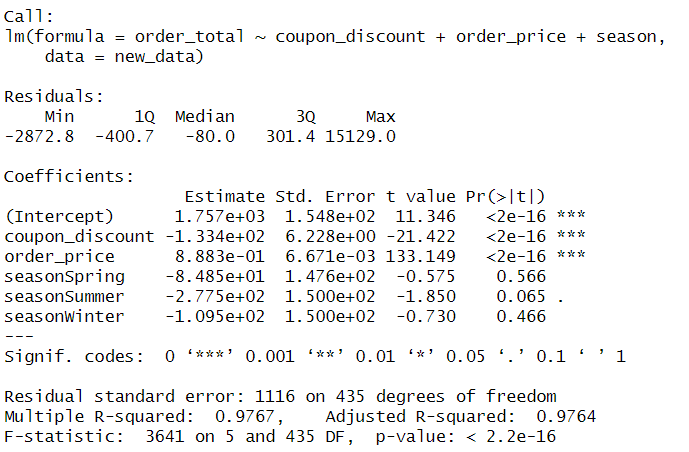
\includegraphics[width = 0.6\textwidth]{IMAGES/42.png}
    \caption{Kết quả khi thực hiện xây dựng mô hình hồi quy bội}
\end{figure}

\textbf{\textit{Nhận xét:}} Từ kết quả phân tích ta thu được:
\begin{equation*}
    \hat{\beta}_0 = 1.757e+03; \hat{\beta}_1 = -1.334e+02; \hat{\beta}_2 = 8.883e-01; 
\end{equation*}
\begin{equation*}
    \hat{\beta}_3 = -8.485e+01; \hat{\beta}_4 = -2.775e+02; \hat{\beta}_5 = -1.095e+02
\end{equation*}
Như vậy, đường thẳng hồi quy ước lượng cho bởi phương trình sau:
\begin{center}
$\widehat{order\_total}$ = $1.757e+03$ + $(-1.334e+02) \times$ coupon\_discount + $(8.883e-01) \times$ order\_price + $(-8.485e+01) \times$seasonSpring + $( -2.775e+02) \times$seasonSumer + $(-1.095e+02) \times$seasonWinter.
\end{center}
Kiểm định các hệ số $\beta_i$:
\begin{itemize}
    \item[+] Giả thuyết H$_0$: $\beta_i = 0$: hệ số $\beta_i$ không có ý nghĩa thống kê.
    \item[+] Đối thuyết H$_1$: $\beta_i \neq 0$: hệ số $\beta_i$ có ý nghĩa thống kê.
\end{itemize}

Ta nhận thấy rằng p-value ứng với các biến seasonSummer, seasonSpring, seasonWinter lớn hơn mức ý nghĩa 5\% nên ta chưa bác bỏ được H$_0$. Vậy hệ số $\beta_i$ ứng với các biến này bằng 0 (không có ý nghĩa thống kê). Tức là các biến này không ảnh hưởng order\_total. Ta sẽ xem xét loại bỏ các biến này ra khỏi mô hình.

Ta xây dựng mô hình model\_2 bỏ đi biến season từ model\_1 (\textbf{Code[219$\to$220]}). 
\begin{figure}[H]
    \centering
    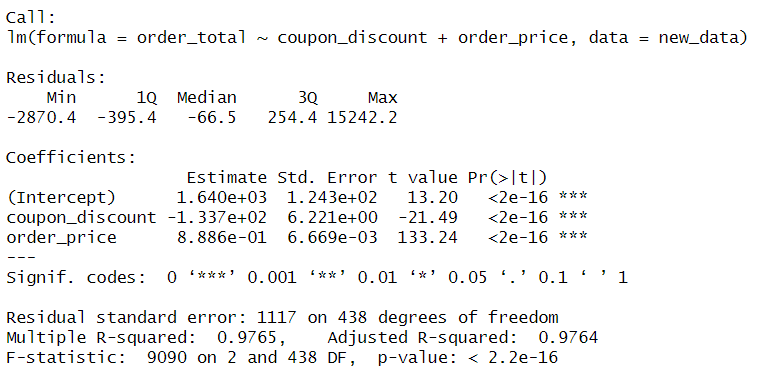
\includegraphics[width = 0.7\textwidth]{IMAGES/43.png}
    \caption{Kết quả khi thực hiện xây dựng mô hình 2}
\end{figure}
So sánh hai model\_1 và model\_2:
\begin{itemize}
    \item[] Giả thuyết H0: Mô hình model\_2 hiệu quả hơn.
    \item[] Đối thuyết H1: Mô hình model\_1 hiệu quả hơn.
\end{itemize}
\textbf({Code[222]}).
\begin{figure}[H]
    \centering
    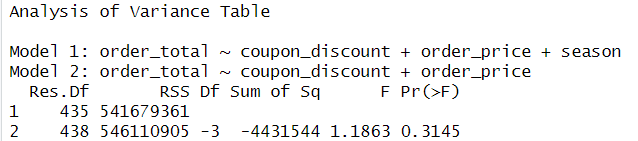
\includegraphics[width = 0.6\textwidth]{IMAGES/45.png}
    \caption{Kết quả khi so sánh hai mô hình 1 và mô hình 2}
\end{figure}
\textbf{\textit{Nhận xét:}} Ta nhận thấy p-value = 0.3145 lớn hơn mức ý nghĩa 5\%, nên ta chưa bác bỏ được H0, vậy nên mô hình model\_2 hiệu quả hơn. Qua việc so sánh ta có thể nhận thấy mô hình model\_2 là mô hình hiệu quả nhất.

Các giả định của mô hình hồi quy: $Y_i  = \beta_0 + \beta_1 X_1 + \ldots + \beta_i X_i + \varepsilon_i,\ i = 1,\ldots n$.
\begin{itemize}
    \item[+] Tính tuyến tính của dữ liệu: mối quan hệ giữa biến dự báo X và biến phụ thuộc Y được giả sử là tuyến tính.
    \item[+] Sai số có kỳ vọng bằng 0.
    \item[+] Phương sai của các sai số là hằng số.
    \item[+] Sai số có phân phối chuẩn. $\varepsilon \sim N(0,\sigma^2)$.
    \item[+] Các sai số $\varepsilon_1, \ldots, \varepsilon_n$ thì độc lập với nhau.
\end{itemize}

Ta thực hiện phân tích thặng dư để kiểm tra các giả định của mô hình (\textbf{Code[224$\to$225]}). 
\begin{figure}[H]
    \centering
    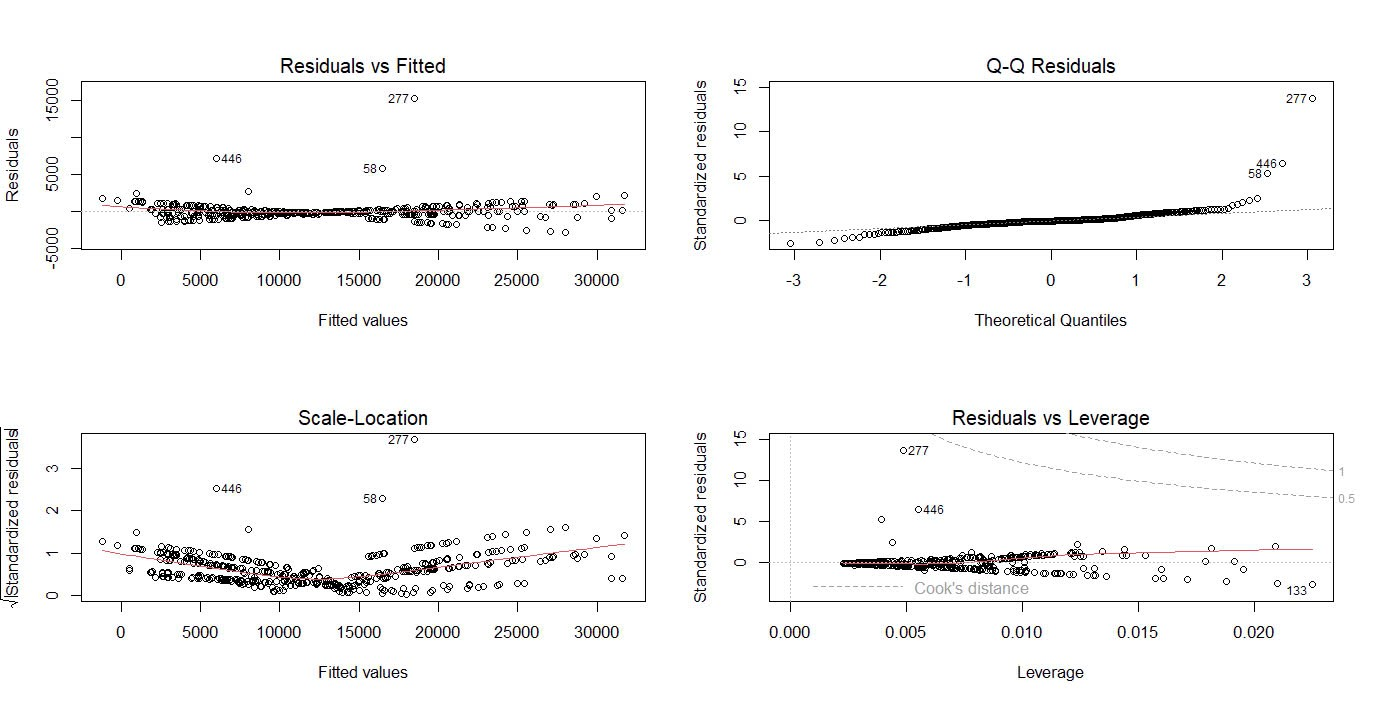
\includegraphics[width = 0.8\textwidth]{IMAGES/50.png}
    \caption{Code R và kết quả khi vẽ đồ thị phân tích thặng dư để kiểm tra các giả định của mô hình}
\end{figure}

\textbf{\textit{Nhận xét:}}

\textbf{Đồ thị 1:} Vẽ các sai số hồi quy tương ứng với giá trị dự báo, dùng để kiểm tra giả định:
\begin{itemize}
    \item[+] Y và các biến độc lập X có quan hệ tuyến tính.
    \item[+] Sai số có kỳ vọng bằng 0.
    \item[+] Phương sai các sai số là hằng số.
\end{itemize}
Dựa vào kết quả cho thấy:
\begin{itemize}
    \item[+] Đường màu đỏ tương đối là đường thẳng nằm ngang nên giả định Y và các biến độc lập X có quan hệ tuyến tính thoả mãn.
    \item[+] Đường màu đỏ tương đối nằm sát đường y = 0 nên ta giả định Sai số có kỳ vọng bằng 0 thoả mãn.
    \item[+] Các giá trị sai số chưa phân tán ngẫu nhiên dọc theo đường màu đỏ, nên giả định Phương sai các sai số là hằng số chưa thoả mãn.
\end{itemize}

\textbf{Đồ thị 2:} Vẽ các sai số hồi quy được chuẩn hoá, dùng để kiểm tra giả định sai số có phân phối chuẩn.

Dựa vào kết quả cho thấy: các quan trắc tương đối nằm trên đường thẳng kỳ vọng phân phối chuẩn nên giả định Sai số có phân phối chuẩn thoả mãn

\textbf{Đồ thị 3:} Vẽ căn bậc 2 các sai số được chuẩn hoá, dùng để kiểm tra giả định Phương sai các sai số là hằng số.

Dựa vào kết quả cho thấy: Các giá trị sai số chưa phân tán ngẫu nhiên dọc theo đường màu đỏ, nên giả định phương sai các sai số là hằng số chưa thực sự thoả mãn.

\textbf{Đồ thị 4:} Vẽ ra những điểm có gây ảnh hưởng cao trong bộ dữ liệu cụ thể là các điểm 446,227. Tuy nhiên, không điểm nào vượt khỏi đường Cook's distance. Vì vậy, ta không cần loại bỏ các điểm khỏi dữ liệu.

 Mô hình hồi quy tuyến tính về sự ảnh hưởng các nhân tố lên biến tổng chi phí đặt hàng (order\_total) = 1.640e+03 + 8.886e-01 x order\_price  + -1.337e+02 x coupon\_discount \\

Hệ số xác định hiệu chỉnh (Adjusted R-squared): $R^2$ hiệu chỉnh  = 0.9764  nghĩa là 97.64\% sự biến thiên trong tổng chi phí đặt hàng (order\_total) được giải thích bởi các biến độc lập.


